\section{Geometrie}
\subsection{Kurvendarstellungen}
Parameterdarstellung: $\vec{c}(t) = (x(t); y(t); ...) \qquad (t \in \text{Intervall})$\\
Explizite = Funktionsdarstellung: $y = f(x)$\\
Implizite Darstellung: $y - x = 0$ 


\subsection{Umrechnung}
\todo{$r = \sqrt{x^2 + y^2}$; $x = r\cos\phi$; $y = r\sin\phi$\\
Vektoriell: $f'(x_0) = \frac{\dot y}{\dot x}$ \bronstein{}
}

\subsubsection{Differential}
Bei der Umrechnung des Differentials kann folgende Logik übernommen werden: $dy = f'(x) \cdot dx$. ACHTUNG: Grenzen des Intervalls müssen ersetzt werden.

\subsection{Kurven zweiter Ordnung}
Kreis: $x^2 + y^2 = r^2 \qquad (r \geq 0)$\\
Ellipse: $\left(\frac{x - x_0}{a}\right)^2 + \left(\frac{y - y_0}{b}\right)^2 = r^2$\\
Hyperbel: $\frac{(x - x_0)^2}{a^2} - \frac{(y - y_0)^2}{b^2} = 1$\\
~\\
Limacons/Herzkurve: $r = a(1 + \cos\phi)$

\subsection{Steigung und Tangentenberechnung}
\subsubsection{Tangentengleichung}
Spezialfall von Tayler-Polynom mit Entwicklungspunkt $a$:
\[Tn_2(x, a) = \hat{f}(x) = f(a) + f'(a)\cdot(x - a)\]
Die Normale (orthogonal am Entwicklungspunkt $a$); Steigung berechnen mit $f'(a) \cdot m_n = -1$ und $y = m_n \cdot x + b$ berechnen.

\subsubsection{Steigung}
\todo{\textbf{Implizit} $y' = \frac{b^2}{a^2}\cdot \frac{x}{y}$\\
	\textbf{Vektor} $y' =$ \\
	\textbf{Polar} $y' = \frac{r'\sin\phi + r\cos\phi}{r'\cos\phi - r\sin\phi}$}

\subsection{Kurven}
\todo{
	\label{bronstein:s60}
	\bronstein{S60}\\
	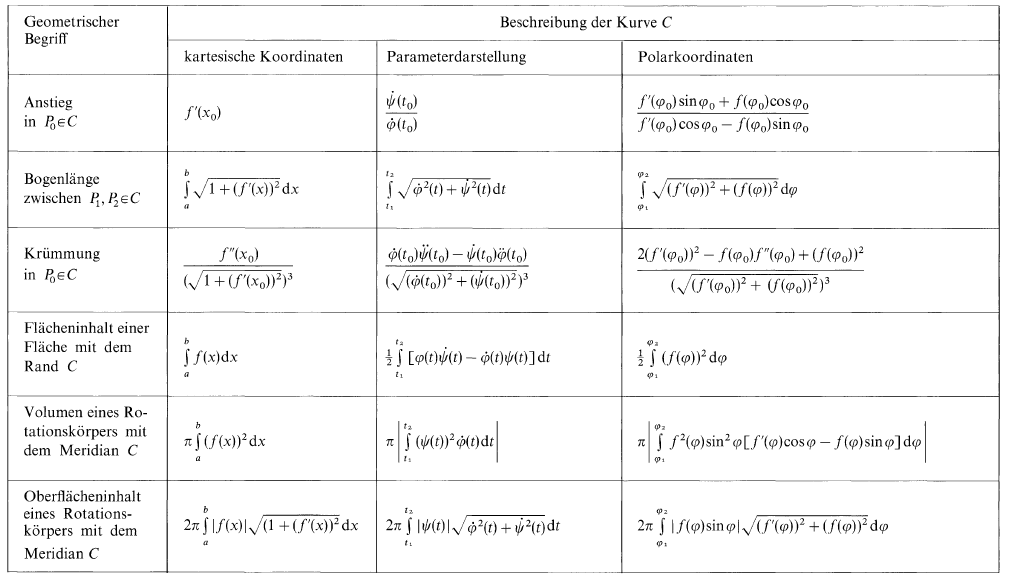
\includegraphics[width=\columnwidth]{Images/FoBronstein}
}

\noindent Bogenlänge $l = \int\limits_{x_1}^{x_2}\sqrt{1 + f(x)^2}dx$\\
\noindent Kurvenfläche $F = \frac{1}{2}\int\limits_{a}^{b}r^2(\phi)d\phi$

\subsection{Rotation}
\todo{Vektor/Polar. Siehe \ref{bronstein:s60}}
\noindent Volumen $V_x=\pi\int f(x)^2dx$

\noindent Oberfläche $O_x = 2\pi\int_{a}^{b}\left|f(x)\right|\sqrt{1 + f(x)^2}dx$

\subsubsection{Drehachse}
\todo{Umkehrfunktionen und Grenzen anpassen! (Grenzen durch Umkehrfunktion herausfinden). Siehe \ref{bronstein:s60}}

\subsection{Krümmungen}
$K(x_0) = \frac{d\alpha}{ds} = \frac{f''(x_0)}{\sqrt{1 + f'(x)^2}^3}$